\section{Spatial Effects}

There are many spatial effect that can exist here because of the diffusion term in the biomass.
We now try observing any differences in the behaviour of the system based on spatially different initial conditions.
This will show if there is any noticible differences in the behaviour of the system based solely on the placement of initial biomass.
%!% At some time I should do the same 6-panel plot I made in the typical simulation here, it'll probably be pretty good...
There will be two methods to compare the different simulations: visually and by monitoring the amount of $CO_2$ produced.
The visual inspection is a logical comparison to use, the $CO_2$ is chosen since it essentially provides a measure of the activity in the system.
The $CO_2$ is also used in the experiments conducted in \cite{dumitrache2014understanding}.
Looking at the $CO_2$ production, a lumped measurement of the biomass activity, shows whether local spatial effects change the global reactor scale behaviour.
%!%If there is no difference then the ODE model (which ignores spatial effects due to the lack of spatial discritization??) can be used accuratly to model the biomass growth.

To measure the difference, two simulations will be run with varying initial conditions.
One simulation will have the initial condition evenly spread along one side of the region.
The other will have all the initial condition clumped in single corner.
This will replicate the two possible extremes for the location of biomass.

%!% (An alternative to add would be to run 10+ test with 'random' initial condition along one side of the boundar and see if there are noticble differences in the set.
%!% Maybe something like standard deviation, error, and showing all the final visuals at t=20 for example.)

Since the only difference is the initial conditions, and since an equal start must be assured, the selection of initial condition is important.
The equally dispersed initial condition needs to have as much surface area exposed as reasonably possible.
To this end, $num$ spherical innoculation points, equidistance from each other, are used along the $y=0$ side of $\Omega$.
Here we use $(x_e, y_e)$ as the center of the evenly distributed innoculation points.
The value of $(x_e, y_e)$ depends on the number of points chosen for the simulation.
Each spherical innoculation point is computed as,
%!% Make a schematic that shows X circles with an unknown distance between them and then show the calculation for that distance and from that get an equation for the sequence of points to be used.
\begin{equation}
M(0,x,y) = \frac{-h}{d^2} ((x-x_e)^2 +(y-y_e)^2) + h, \quad M \ge 0.
\end{equation}
Note that $M(0,x,y)$ is for points within circles of radius $d$ centered at $(x_e, y_e)$, otherwise $M(0,x,y) = 0$.
For the substratum we have $C(0,x,y) = 1$ everywhere.

\begin{figure}
  \centering 
  \begin{tabular}{c c}
    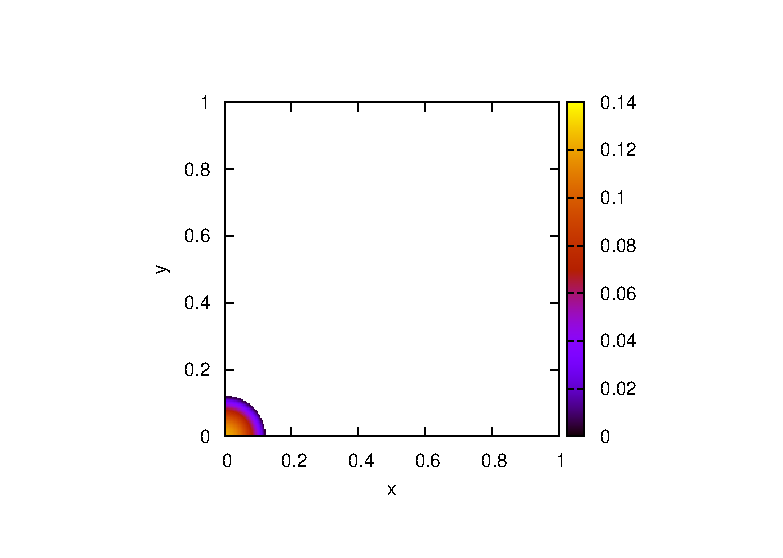
\includegraphics[scale=0.65]{spatial_clump_t0.eps} &
    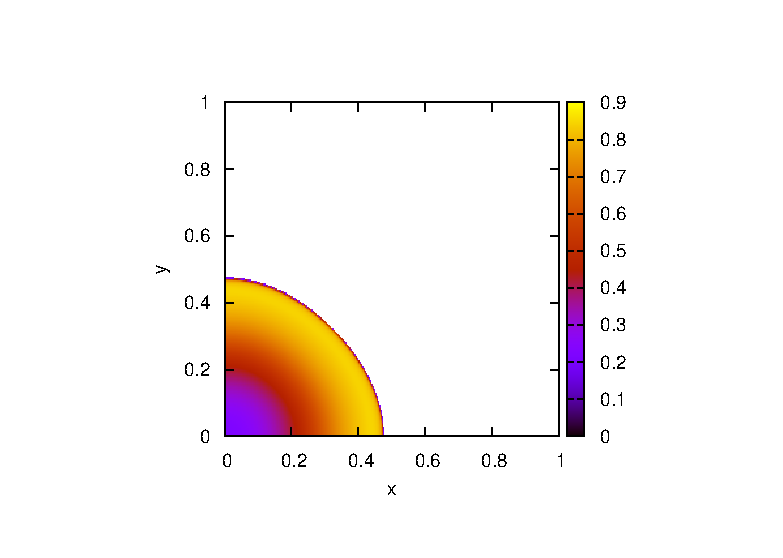
\includegraphics[scale=0.65]{spatial_clump_t16.eps} \\
    (a) & (b) \\
    \includegraphics[scale=0.65]{spatial_clump_t32.eps} &
    \includegraphics[scale=0.65]{spatial_clump_t48.eps} \\
    (c) & (d) 
  \end{tabular}
  \caption{This shows the time evolution for the clumped initial condition at (a) $t=0$, (b) $t=16$, (c) $t=32$, (d) $t=48$.
    Here default parameters are used on a grid size of $513 \times 513$.
    }
  \label{fig:spatial_clump}
\end{figure}

\begin{figure}
  \centering 
  \begin{tabular}{c c}
    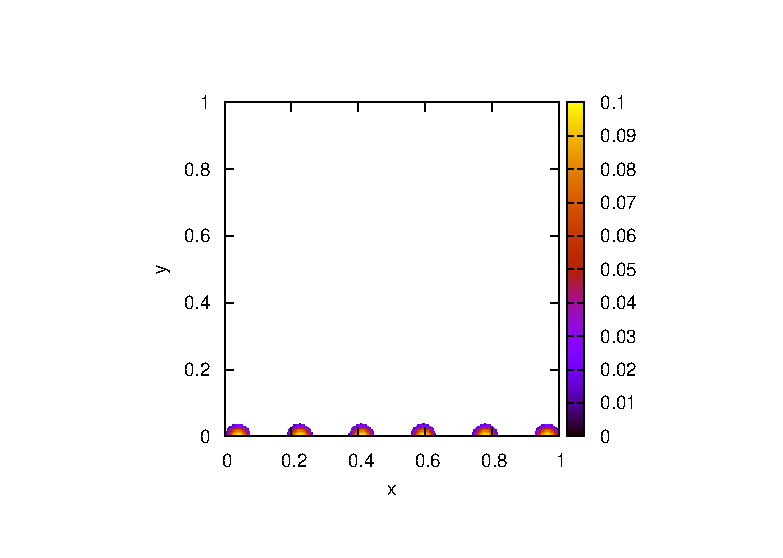
\includegraphics[scale=0.65]{spatial_even_t0.eps} &
    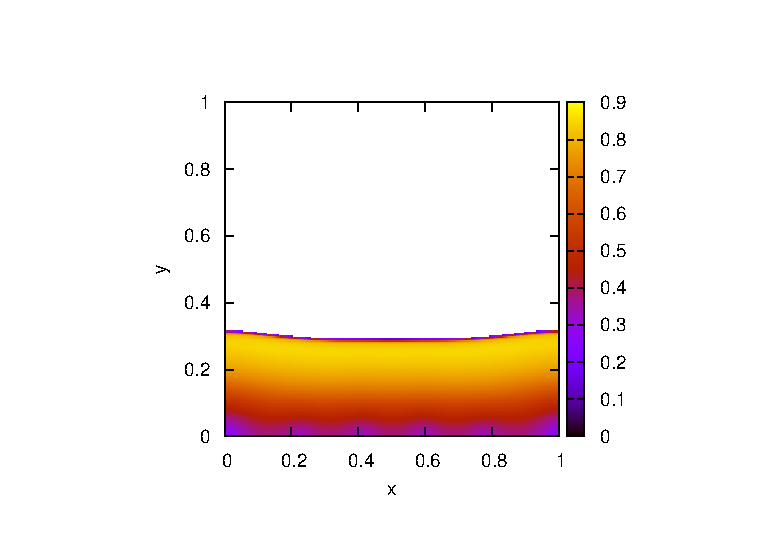
\includegraphics[scale=0.65]{spatial_even_t16.eps} \\
    (a) & (b) \\
    \includegraphics[scale=0.65]{spatial_even_t32.eps} &
    \includegraphics[scale=0.65]{spatial_even_t48.eps} \\
    (c) & (d) 
  \end{tabular}
  \caption{This shows the time evolution for the evenly distributed initial condition at (a) $t=0$, (b) $t=16$, (c) $t=32$, (d) $t=48$.
    Here default parameters are used on a grid size of $513 \times 513$.
    }
  \label{fig:spatial_even}
\end{figure}
For the clumped initial condition, we choose another spherical innoculation point so that it is similar to the evenly distributed initial condition.
Here, we need only a single innoculation point, centered at the corner $(0,0)$.
The choice of innoculation center is so that the initial biomass is as concentrated as possible, while still retaining a spherical shape.
The initial condition for the clumped biomass is as follows, 
\begin{equation}
M = \frac{-1}{(2hd^2\cdot num)^{\frac{1}{3}}} (x^2 + y^2) + (2hd^2\cdot num)^{\frac{1}{3}}.
\end{equation}
Here the coefficents have been chosen so that the two initial conditions have the same amount of biomass.
The value of $num$ is to represent the number of innoculation points in the evenly distributed initial condition.
%Show that they both have the same total amount via calculus

Figure \ref{fig:spatial_clump}-\ref{fig:spatial_even} shows the time evolution of both initial conditions.
Here we arbitrarily select $num = 6$.

\begin{figure}
  \centering
  \begin{tabular}{c}
    \includegraphics[scale=0.9]{spatial_CO2.eps} \\
    (a) \\
    \includegraphics[scale=0.9]{spatial_CO2_total.eps} \\
    (b)
  \end{tabular}
  \caption{A plot of (a) $\mathcal{R}(t)$ and (b) $\mathcal{P}(t)$.
    These are extracted from the same simulation done in the two previous figures.
  }
  \label{fig:spatial_CO2}
\end{figure}

It becomes easier to see the difference between the two spatially difference problems when $CO_2$ production is taken into account.
In Figure \ref{fig:spatial_CO2} it is clear that there is a substantial difference between the $CO_2$ production of both cases.
This shows that the initial distribution of biomass can affect a lumped, global measurement and change the reactor-scale behaviour.
From this, two dimensional models that take spatial consideration at a meso-scale can lead to different results.



%!%Describe that there actually exist a small difference in initial total biomass at t=0 because of how the grid sizes worked out.
%Explain that this gets smaller at more precise grid sizes.
%But that small difference does not explin the massive different in results
